%%%%%%%%%%%%%%%%%%%%%%%%%%%%%%%%%
%%  Descrizione dell'architettura
%%%%%%%%%%%%%%%%%%%%%%%%%%%%%%%%%



\subsection{Metodo e formalismo di specifica}
La descrizione dell'architettura di \proj{} è suddivisa in quattro sezioni:
\begin{itemize}
	\item §\ref{sec:arch_gen}, che illustra gli aspetti generali dell'architettura del software;
	\item §\ref{sec:arch_client}, che descrive l'architettura del \emph{front end} dell'applicazione;
	\item §\ref{sec:arch_server}, che descrive l'architettura del \emph{back end} dell'applicazione;
	\item §\ref{sec:arch_proto}, che descrive il protocollo che lega le due interfacce precedenti.
\end{itemize}
Per ognuna di queste sezioni, procediamo con metodo \emph{top-down} --- dal generale al particolare. utilizziamo dei diagrammi che seguono i formalismi di UML 2.0 e in essi, evidenziamo in colore più scuro le parti dell'architettura che sono di librerie esterne.



\subsection{Descrizione generale} \label{sec:arch_gen}
L'architettura dell'applicazione è suddivisa in due moduli:
\begin{enumerate}
	\item il client, che vive nel browser dell'utente;
	\item il server, che fornisce la pagina dell'applicazione al client e riceve da esso delle richieste di generazione di codice.
\end{enumerate}

Tra le varie qualità desiderabili per la nostra architettura, la progettazione ha perseguito principalmente l'\textbf{estensibilità}. Tale obiettivo è stato raggiunto con due strategie:
\begin{itemize}
	\item in generale, promuovendo le seguenti qualità:
	\begin{itemize}
		\item manutenibilità;
		\item modularità;
		\item semplicità;
		\item basso accoppiamento.
	\end{itemize}
	\item nello specifico, prevedendo le seguenti possibili aggiunte nel futuro:
	\begin{itemize}
		\item Generazione di codice in altri linguaggi target: se i manutentori vorranno generare del codice JavaScript o Python, sarà sufficiente aggiungere dei template per il linguaggio scelto (grazie alla libreria \emph{StringTemplate}) e implementare le interfacce \texttt{Generator} e \texttt{Compiler}.
		\item Diversa compressione del codice generato: attualmente l'applicazione genera un JAR e lo comprime, assieme al file JSON, in formato ZIP; ma si potrebbe facilmente cambiare il formato di compressione in un JAR che contenga egli stesso al suo interno il file JSON.
		\item Persistenza dei dati del diagramma che arrivano in input al \emph{back end}: si potrebbe voler mantenere un database di utenti dell'applicazione, ognuno con i propri diagrammi mantenuti nel server a tempo indefinito; per questo, basta fornire l'indirizzo della risorsa JSON, che attualmente non viene eliminata dal server. % (oppure per ora potremmo eliminarla...)
		\item Persistenza del programma generato: si potrebbe voler mantenere anche il codice generato, come il diagramma di input; per fare ciò, basta garantire al client il carattere persistente della risorsa fornita (badando però a non eliminarla dal server). % (per ora la eliminiamo?)
%		\item Diverso formato per i diagrammi in input: si potrebbe voler ricevere dei dati da un client esterno, anziché in JSON (e.g. disegnatori di diagrammi UML come Astah); sarà sufficiente modificare il package \texttt{parser}.
		\item Modifica degli stereotipi UML offerti: gli stereotipi sono disaccoppiati dalla pagina principale dell'applicazione, in quanto vengono forniti al client separatamente dalla pagina stessa, in modo asincrono.
	\end{itemize}
\end{itemize}



\subsection{Architettura del client} \label{sec:arch_client}
Il \emph{front end} di \proj{} è una \emph{Single Page Application} (\gloss{SPA}) scritta in HTML5, CSS3 e JavaScript.

L'\texttt{head} (intestazione) della pagina HTML contiene dei riferimenti a:
\begin{itemize}
	\item uno script JavaScript che sfrutta \requirejs per risolvere le dipendenze tra le varie librerie JavaScript che utilizziamo;
	\item i fogli di stile CSS di alcune librerie;
	\item il foglio di stile CSS della pagina.
\end{itemize}

Il \texttt{body} (corpo) della pagina HTML si compone di pochi blocchi:
\begin{itemize}
	\item dei tag \texttt{div} contenenti i menù laterali da cui selezionare gli strumenti e gli elementi per interagire con i diagrammi;
	\item un tag \texttt{svg} (identificato dall'\texttt{id} \emph{paper}) che contiene, di volta in volta, il diagramma delle classi o il diagramma di un metodo particolare.
\end{itemize}
Alla ricezione della pagina da parte del client, lo script JavaScript popola il tag \texttt{svg} (inizialmente vuoto) con un diagramma delle classi vuoto.

L'architettura del client è suddivisa in tre moduli, come in figura \ref{fig:client_pkg}:
\begin{itemize}
	\item \texttt{model}, che organizza la logica sottostante i diagrammi;
	\item \texttt{view}, che gestisce l'interfaccia grafica;
	\item \texttt{collection}, che raggruppa in una collezione più model, come per tutti i diagrammi creati. % <<< ?
\end{itemize}

\texttt{model} contiene i vari tipi di celle dei diagrammi: elementi del diagramma delle classi, collegamenti tra essi, stereotipi per giochi da tavolo e, infine, elementi dei diagrammi a blocchi. % ...

\texttt{view} offre la classe \texttt{ProjectView}, che rappresenta l'area di disegno principale dell'applicazione. Attorno ad essa sono presenti dei menù: \texttt{DetailsView} visualizza tutti i campi di un elemento o di un collegamento tra elementi e ne permette la modifica; \texttt{NewCellView} visualizza tutti i possibili tipi di elementi e collegamenti che si possono inserire in un diagramma. Tutta l'interfaccia grafica è orchestrata da una \texttt{AppView}, che crea una \texttt{ProjectView}, una \texttt{DetailsView} e una \texttt{NewCellView}.

\texttt{collection} contiene soltanto la classe \texttt{DiagramCollection}, che compone in una collezione più oggetti \texttt{Graph} (tipo definito da \jointjs). Ognuno di questi oggetti è un diagramma (a classi o a blocchi).

% diagramma dei package del client
\begin{figure} \label{fig:client_pkg}
	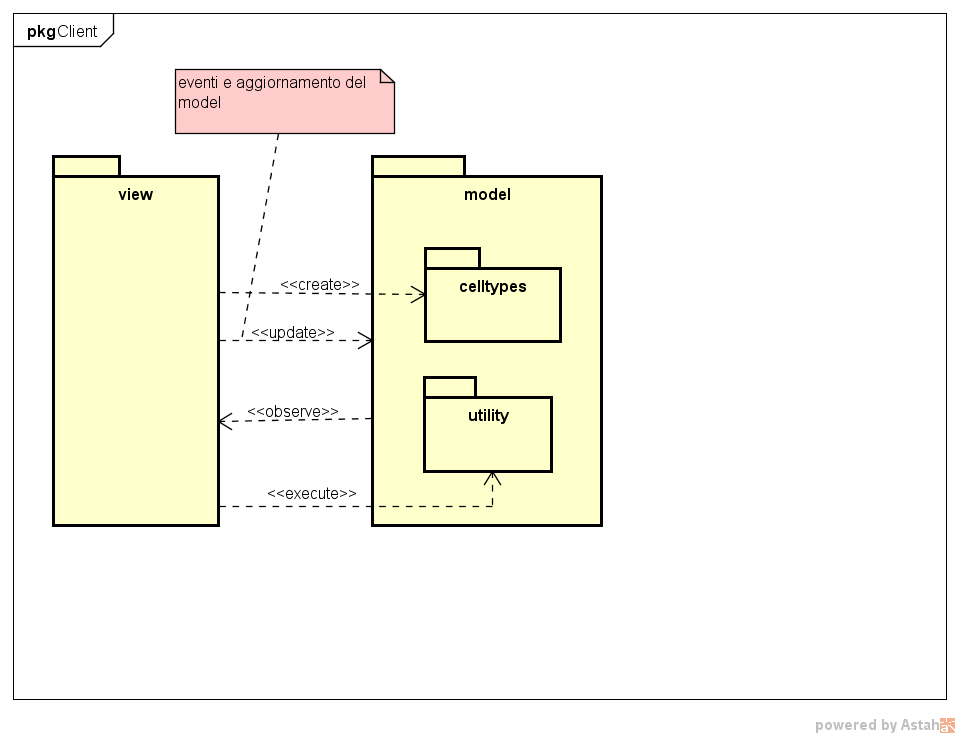
\includegraphics[scale=0.5]{img/client_pkg}
	\caption{Architettura del client.}
\end{figure}

\subsubsection{Diagrammi}
I due tipi di diagrammi visualizzabili sul client sono: diagramma delle classi; diagramma di attività.

	\paragraph{Diagramma delle classi}
Il diagramma delle classi è un normale diagramma UML che offre un sottoinsieme dei formalismi definiti dal relativo standard, ispirato al \emph{20 percent of UML that helps you do 80 percent of your work} di cui parla Martin Fowler in \emph{UML Distilled}. L'editor ad esso relativo propone all'utente anche delle funzionalità aggiuntive fra cui la possibilità di marcare le classi create con dei particolari stereotipi già definiti. Questi rappresentano un insieme di vincoli logici e semantici che l'utente deve rispettare nel popolare la classe, come, ad esempio, metodi da scriversi obbligatoriamente o l'impossibilità di inserire campi dati.
	\paragraph{Diagramma delle attività}
La seconda tipologia di diagramma viene da noi chiamata "diagramma delle attività" per l'affinità che la lega al corrispettivo formalismo di modellazione dell'UML anche se in realtà ne rappresenta una profonda revisione. L'editor mette a disposizione dell'utente una serie di blocchi da comporre per popolare il corpo di uno specifico metodo, ognuno dei quali legato - anche nominalmente - a statement o formalismi tipici dei linguaggi di programmazione. Vi è la possibilità di scegliere fra blocchi variabili per assegnazioni o dichiarazioni, blocchi metodi per la loro invocazione, blocchi return per uscire dal metodo in esame, blocchi if/else per le ramificazioni decisionali, blocchi while e for che rappresentano i relativi cicli iterativi e blocchi custom per inserire codice senza alcun vincolo a monte.
In generale l'utente compone questi elementi inserendoli uno di seguito all'altro, libero di spostare in una nuova posizione all'interno della sequenza le unità desiderate.
All'interno del corpo dei blocchi while, for e if/else è inoltre possibile inserire una qualsiasi sequenza dei blocchi precedentemente elencati in modo tale da aumentare i livelli di innestamento delle varie istruzioni e quindi, in generale, la complessità del metodo stesso.
È inoltre possibile corredare ogni blocco con un commento che ne illustri il "contratto" in modo tale da poter mantenere una visione ad alto livello del flusso logico delle azioni definite anche nel caso in cui si decida di visualizzare in formato ridotto i diversi elementi.




\subsection{Architettura del server} \label{sec:arch_server}
Il server offre tre servizi:
\begin{enumerate}
	\item fornisce al client la pagina HTML dove disegnare i diagrammi;
	\item restituisce l'elenco degli stereotipi esistenti all'interno del server e utilizzabili dal client;
	\item elabora un file JSON in arrivo dal client e gli fornisce l'applicazione generata a partire da tale file.
\end{enumerate}
Questi tre servizi rispettano lo stile architetturale REST (come spiegato più avanti nella sezione \ref{sec:arch_proto}).

Il primo servizio è una semplice pagina HTML, fornita normalmente da Tomcat e arricchita di codice Javascript.

Il secondo e il terzo servizio, invece, sono un programma Java che genera due \emph{servlet}; il programma è organizzato nei seguenti package, come illustrato in figura \ref{fig:server_pkg}:
\begin{itemize}
	\item \textbf{\texttt{controller}} rappresenta il nucleo del \emph{back end}; un \texttt{RequestHandlerController} si occupa di generare le due \emph{servlet} Java, usando \emph{Spring}.
	\item nel package \textbf{\texttt{parser}}, la classe \texttt{Parser} si occupa di convertire il file JSON ricevuto in un oggetto Java di tipo \texttt{ParsedProgram}. Questo oggetto Java rappresenta il programma che l'utente vuole generare; esso si compone di oggetti \texttt{ParsedType} (cioè i tipi definiti dall'utente: gli elementi del diagramma delle classi), i quali si possono comporre di oggetti \texttt{ParsedAttribute} e \texttt{ParsedMethod}; quest'ultimo tipo si compone a sua volta di oggetti \texttt{ParsedInstruction} e così via fino ad arrivare alle istruzioni “atomiche”, come per esempio un \texttt{ParsedReturn}.
	\item \textbf{\texttt{project}} non è altro che il package che organizza i tipi elencati al punto precedente, tutti discendenti da \texttt{ParsedElement}. Inoltre, questo package offre una classe \texttt{ElementFactory}. % che non ho capito cosa fa
	\item \textbf{\texttt{generator}} presenta al suo interno l'interfaccia \texttt{Generator}; le classi che la estendono si occupano di popolare i template \emph{StringTemplate} di un particolare linguaggio di programmazione (\texttt{JavaGenerator} genera codice sorgente Java) e scrivere il risultato su disco. \texttt{GeneratorAssembler} fornisce la giusta implementazione \texttt{Generator}, grazie a un file di configurazione XML e a \emph{Spring}.
	\item \textbf{\texttt{template}} è il package che organizza i template per linguaggio: dall'interfaccia \texttt{Template} discende, ad esempio, \texttt{JavaTemplate}. Anche questo package presenta una classe che si occupa di fornire la giusta implementazione di \texttt{Template}: \texttt{TemplateAssembler}, dipendente anch'esso dal file di configurazione XML.
	\item \textbf{\texttt{stereotype}} espone una classe che recupera da disco i vari template di ogni stereotipo implementato.
	\item \textbf{\texttt{compiler}} presenta l'interfaccia \texttt{Compiler}, le cui implementazioni specifiche (per un certo linguaggio target) compilano il codice sorgente non eseguibile in un programma eseguibile (che viene poi scritto su disco); \texttt{JavaCompiler}, ad esempio, compila codice sorgente Java in \emph{bytecode} per la JVM (Java Virtual Machine) e compatta il codice in un file JAR eseguibile. Anche questo package presenta un \texttt{CompilerAssembler} (dipendente dal file di configurazione XML) che si occupa di fornire la giusta implementazione di \texttt{Compiler}.
	\item \textbf{\texttt{utility}} espone classi di utilità per il programma, come ad esempio una classe \texttt{Compressor} che comprime l'output di un \texttt{Compiler} in formato ZIP. % è pulito tenere un package con un nome così generico?
\end{itemize}

% >>> diagr. dei package del server
\begin{figure} \label{fig:server_pkg}
	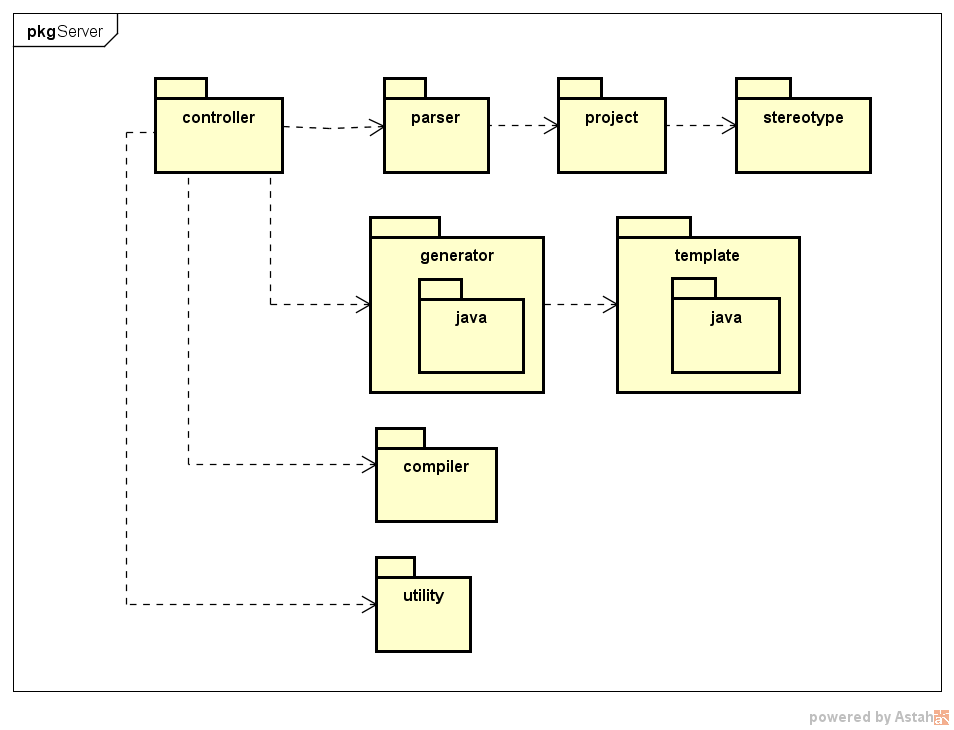
\includegraphics[scale=0.5]{img/server_pkg}
	\caption{Architettura del server.}
\end{figure}



\subsection{Protocollo di comunicazione client-server} \label{sec:arch_proto}
I tre servizi offerti dal server (ottenere la pagina HTML; recuperare stereotipi UML; ottenere l'applicazione generata) seguono lo stile architetturale REST:
\begin{itemize}
	\item La richiesta per ottenere la pagina HTML usa il metodo HTTP GET; la pagina è quindi \emph{cachable} (i router tra client e server possono decidere di ottimizzarne la fornitura).
	\item Il file JSON viene spedito con il metodo HTTP POST, che permette la persistenza di tale file nel server; la persistenza del file JSON è indifferente alla nostra applicazione ma ne aumenta l'estensibilità, in quanto un giorno i manutentori potrebbe voler offrire un servizio di condivisione dei diagrammi disegnati oppure un database di utenti che abbiano i propri diagrammi sul server.
	\item Ognuno dei tre servizi (pagina HTML, recupero di stereotipi e generazione di codice) è una risorsa distinta: questo disaccoppia i due servizi, aumentando ancora la manutenibilità del sistema.
	\item La richiesta per ottenere la pagina HTML è per forza idempotente: lo stato del server non può influire su una pagina statica. %Neanche il recupero di stereotipi dipende dallo stato del server, dato che gli stereotipi sono contenuti in file statici. % <<< o forse no?
	\item La richiesta di generazione di codice è idempotente: l'unica dipendenza esterna al programma è il file JSON, che viene passato dal client.
\end{itemize}

\begin{figure} \label{fig:protocol}
	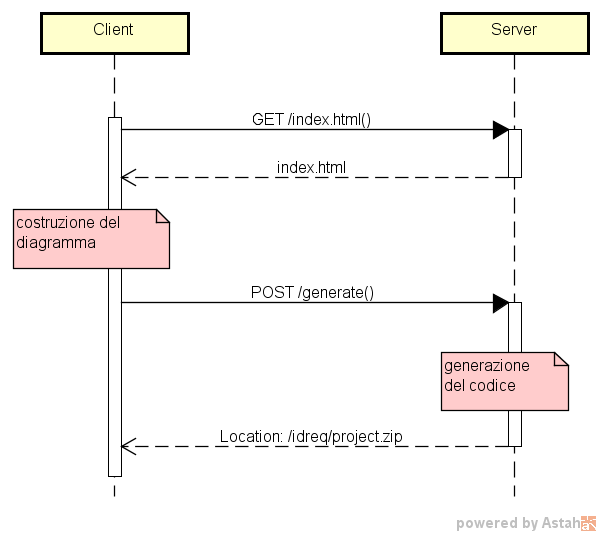
\includegraphics[scale=0.66]{img/http}
	\caption{Possibile interazione tra client e server.}
\end{figure}

\subsubsection{Pagina HTML}
\begin{itemize}
	\item risorsa: \texttt{/index.html};
	\item metodo: GET;
	\item utilizzo: il client richiede al server la pagina principale dell'applicazione web.
\end{itemize}

\subsubsection{Stereotipi UML}
\begin{itemize}
	\item risorsa: \texttt{/stereotypes};
	\item metodo: GET;
	\item utilizzo: il client richiede al server gli stereotipi disponibili.
\end{itemize}

\subsubsection{Generazione del codice}
\begin{itemize}
	\item risorsa: \texttt{/generate};
	\item metodo: POST;
	\item utilizzo: il client richiede al server di generare il codice relativo al diagramma creato, mandandogli il file JSON del diagramma e ricevendo l'indirizzo della risorsa contenente il codice generato.
\end{itemize}

% ci sarebbe da fare pure una cosa simile per il recupero degli stereotipi
